\chapter{Design}

In this chapter, we lay out the requirements for our implementation of Wasm containers in Apache OpenWhisk. Then we describe and discuss our implementation and the trade-offs involved.

\section{Requirements}

\subsection{Apache OpenWhisk}

In order to understand the requirements for our Wasm-flavored OpenWhisk, we need to understand the design of OpenWhisk itself first.

\begin{figure}
    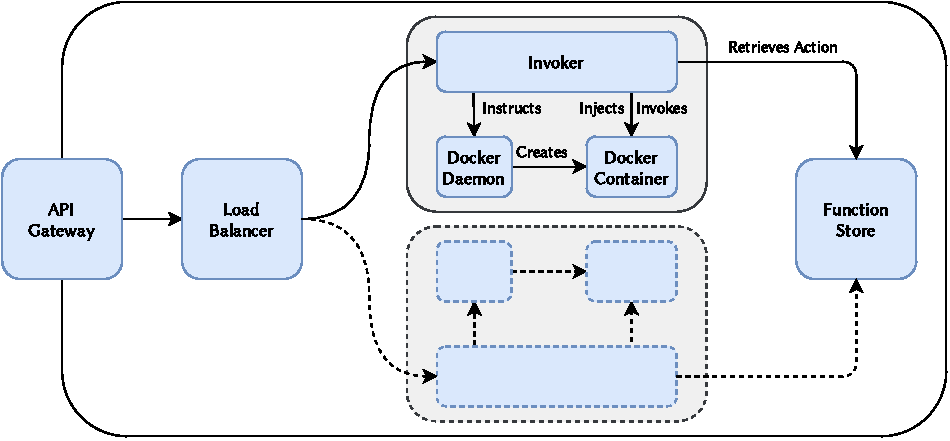
\includegraphics{figures/OpenWhiskActionInvocationFlow.pdf}
    \caption{Action invocation flow in Apache OpenWhisk based on the source code and documentation \cite{OpenWhiskSystemDesign}. Potentially many Invokers can exist in this setup.}
    \label{fig:openwhisk-action-invocation-flow}
\end{figure}

Figure \ref{fig:openwhisk-action-invocation-flow} sketches the design of OpenWhisk. Users interact with it through its API Gateway, which consists of \inl{nginx}, mostly for SSL termination, and the \inl{Controller}, which implements the main logic. It handles the creation of actions, OpenWhisk's name for serverless functions, authentication and authorization as well as invoking the action.
In the latter case, the controller uses its load balancer to determine which Invoker should handle the request, and publishes the request to an Apache Kafka queue, which the invoker is subscribed to. The controller and its load balancing take a central role in OpenWhisk, but in our figure it is represented by the API Gateway and the Load Balancer only, simply because we will not be modifying this part.
Our focus is on the Invoker. It is the part of OpenWhisk responsible for \emph{invoking} the action. A number of steps are involved in that process \cite{OpenWhiskSystemDesign}.

\begin{enumerate}
    \item It retrieves the action's code and execution permissions from an Apache CouchDB database, where the Controller stored it during action creation. 
    \item It instructs the local Docker daemon to start a new container, based on the runtime that the action needs to execute. This would be a \inl{openwhisk/action-nodejs-v10} image for JavaScript actions but could also be a generic black-box image (\inl{openwhisk/dockerskeleton}), that can execute any binary, such as one written in Rust or C.
    \item Finally, it injects the action's code into the container, invokes it with the given parameters and returns the result \cite{OpenWhiskSystemDesign}.
\end{enumerate}

Because OpenWhisk supports many runtimes and even the mentioned black-box image, it needs a common protocol to communicate with all of them. The just-described step 3 is the gist of that protocol. Each runtime needs to implement a \inl{/init} endpoint, where it receives the code and takes whatever steps necessary to make it ready for execution. Thus, over a containers life cycle, this endpoint is called exactly once. Afterwards, the \inl{/run} endpoint can be called multiple times to execute the action \cite{OpenWhiskSystemDesign}.

That implies that the container isn't destroyed immediately after it has been invoked once. Indeed, OpenWhisk uses various optimizations of the described flow, in order to improve the system's performance. Among those are pre-warming containers or keeping the container running for some time after it has been invoked, before it is removed.
We will explore those optimizations in more depth later, to compare them to the optimizations in our Wasm runtime to better see where they coincide and differ \cite{OpenWhiskSystemDesign}.



